\section{Zeiterweiterte Netzwerke}

Unser Ziel ist ein polynomielles Approximationsschema für Quickest-Flow-Probleme.
Die Idee dabei ist, ein Netzwerk $\graph$ in ein \term{zeiterweitertes Netzwerk}
umzuwandeln. Dazu werden für jeden Zeitschritt Kopien der Knoten von $\graph$
angelegt. Dabei gibt die Zeitkomponente den Zeitpunkt eines Flusses an. Daher
werden in dem neuen Graph zwei Knoten genau dann verbunden, wenn die Knoten
im ursprünglichen Graphen durch eine Kante $e \in \A$ verbunden gewesen sind und
sie $\tau(e)$ Zeitschritte entfernt sind. Zusätzlich müssen wir noch Kanten
zwischen den einzelnen Zeitschritten der Quellen und Senken einfügen, damit
der Fluss auch am Ende der Zeit des Flusses verfügbar ist, denn wir werden
die Kopien der Senken zum Zeitpunkt $T-1$ als neue Senken erklären.
% BjH: Der letzte Satz ist kaum verst\"andlich.

Wir nehmen dabei an, dass die Zeiten ganzzahlig sind. Dies ist durch Skalierung
der Zeit auf die gewünschte Genauigkeit für Anwendungen problemlos möglich.

\begin{definition}[Zeiterweitertes Netzwerk]
    Sei $(\graph, \tau)$ ein Netzwerk mit $\tau(e) \in \N$ für alle $e \in \A$
    und $T \in \N$. Setze $\timeDom = \{0, 1, \ldots, T-1\}$.
    Wir definieren damit das \term{zeiterweiterte Netzwerk} $\tExp{T} = (V^T, \A^T)$
    mit
    \begin{itemize}
        \item $V^T = V \times \timeDom$ (schreibe $v_t = (v, t)$ und
            $V_t = \{v_t \in V^T\}$)
        \item $\A^T = \setDef{e_t = (v_t, u_{t + \tau(e)})}
                        {e = (v, u) \in \A \text{ und } t, t + \tau(e) \in \timeDom}
                    \cup H$ \\
            mit „\term{holdover arcs}“ bzw. \term{Speicherkanten} \\
            $H = \setDef{(v_t, v_{t+1})}
                        {v \in S_i \text{ und } t, t + 1 \in \timeDom}$
        \item $\func{u^T}{\A^T}{\REx = \R \cup \{\infty\}}$ mit
                $u^T(e_t) = \begin{cases}
                    u(e)    &, e_t \not\in H \\
                    \infty  &, e_t \in H
                \end{cases}$
        \item $\func{c^T}{\A^T}{\R}$ mit
                $c^T(e_t) = \begin{cases}
                    c(e)    &, e_t \not\in H \\
                    0       &, e_t \in H
                \end{cases}$
        \item $S_i^{+,T} = \setDef{v_0 \in V^T}{v \in S_i^+}$, \\
                $S_i^{-,T} = \setDef{v_{T-1} \in V^T}{v \in S_i^-}$ und damit \\
                $S_i^T = S_i^{+,T} \disjUnion S_i^{-,T}$
% BjH: Hier fehlt immer noch die Definition von $i$. $i$ wurde zwar oben schon eingef\"uhrt, aber diese Definition definiert sich alle Symbole erneut.
    \end{itemize}
    Sollte Speicher an Knoten $V \setminus S$ zugelassen sein, dann müssen analog
    zu $H$ weitere Speicherkanten eingefügt werden.
\end{definition}

\begin{remark}
    Da in Netzwerken $\inEdges(s) = \emptyset$ für alle $s \in S_i^+$ und
    $\outEdges(t) = \emptyset$ für alle $t \in S_i^-$ (d.h. Quellen und Senken
    können keine inneren Knoten auf Flüssen sein), kann in der obigen Definition
    auch $\REx$ durch $\R$ ersetzt werden, wenn man die Kapazität der
    Speicherkanten $(v_t, v_{t+1}) \in H$ größer oder gleich $|D_i(v)|$ für
    $v \in S_i$ wählt. Wenn der Fluss diesen Bedarf übersteigen darf,
    muss die Kapazität entsprechend größer gewählt werden.
\end{remark}

\begin{example}
    Wir wollen uns ein einfaches Beispiel für ein zeiterweitertes Netzwerk 
    ansehen. Dazu sehen wir uns \figRef{ex_time_expanded_1} an. In dem
    Netzwerk deklarieren wir nur $s$ als Quelle und $t$ als Senke:
    $S^+ = \{s\}, S^- = \{t\}$.

    \begin{figure}[H]
    \centering
    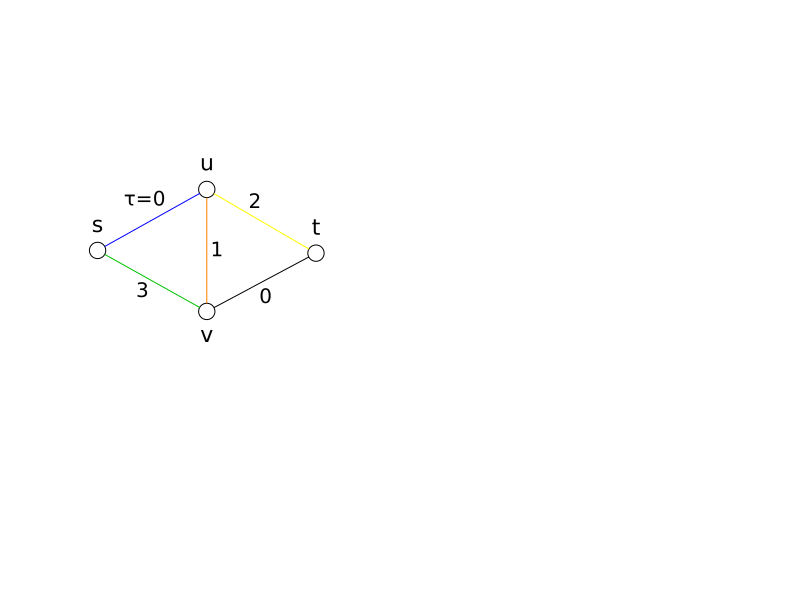
\includegraphics[width=0.5\textwidth]{ex_time_expanded_1}
    \caption{Awesome Image}
    \label{fig:ex_time_expanded_1}
    \end{figure}

    Wir betrachten $T = 6$ und damit $\timeDom = \{0, \ldots, 5\}$. An den
    Kanten sind die Zeiten $\tau$ notiert. Wir nehmen außerdem an, dass
    an dem Knoten $u$ Speicher zugelassen ist. Dann ergibt sich
    des Netzwerk $\tExp{T}$ in \figRef{ex_time_expanded_2}.

    \begin{figure}[H]
    \centering
    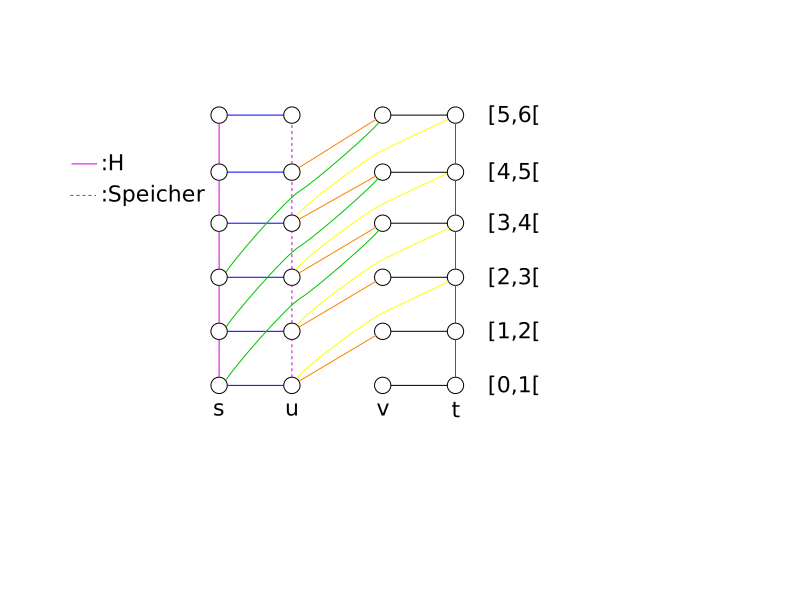
\includegraphics[width=0.7\textwidth]{ex_time_expanded_2}
    \caption{Awesome Image}
    % BjH: Arbeitstitel hier und bei einigen folgenden Bildern ersetzen.
    \label{fig:ex_time_expanded_2}
    \end{figure}
\end{example}

Da wir dynamische Flüsse mit Hilfe von Algorithmen für statische Flüsse
konstruieren wollen, müssen wir zwischen Flüssen $f$ in $\graph$ und
Flüssen $x$ in $\tExp{T}$ wechseln können:

\begin{lemma}\label{lem:static_dyn_conv}
    Ein statischer Fluss $\func{x_i}{\A^T}{\R_+}$ in $\tExp{T}$ entspricht einem
    dynamischen Fluss $\func{f_i}{\A \times \ropen{0,T}}{\R_+}$ in $\graph$
    mit gleichem Flusswert und Kosten und umgekehrt. Dabei gilt:
    \begin{enumerate}
        \item $f_i(e,t) := x_i(e_{\lfloor t \rfloor})$ und
        \item $x_i(e_t) := \int_t^{t+1} f_i(e, \theta) \: d\theta$
    \end{enumerate}
\end{lemma}

Dieser Sachverhalt ist zwar sehr einfach, hat allerdings das Problem, dass das
Netzwerk $\tExp{T}$ sehr groß wird. Denn $|V^T| = |V| \cdot |\timeDom| = n \cdot T$.
Da aber $T$ in der Größe $\log T$ kodiert wird, hängt $V^T$ nicht mehr polynomiell
von der Eingabe ab.

Die Idee ist nun, das Netzwerk $\tExp{T}$ wieder zu verkleinern, so dass es
eine polynomielle Größe erreicht, indem unnötige Zeitschritte entfernt werden.
Das führt zu den \term{skalierten Netzwerken}:

\begin{definition}\label{def:red_network}
    Sei $(\graph, \tau)$ Netzwerk und $0 < \Delta$, so dass $T/\Delta \in \N$
    und $\tau(e)/\Delta \in \N$ für alle $e \in \A$. Wir setzen
    $\tau' := \tau/\Delta$ und damit
    $\redNetw{T}{\Delta} := \tExp{T/\Delta}$ für $(\graph, \tau')$.
    
    Ein Knoten $v_t$ entspricht dann einem Zeitverlauf im Intervall
    $\ropen{t \Delta, (t+1) \Delta}$. Daher müssen die Kosten und Kapazitäten
    auf $c' := c \cdot \Delta$ und $u' := u \cdot \Delta$ korrigiert werden.
\end{definition}

\begin{lemma}\label{lem:reduced_static_dyn_conv}
    Sei $0 < \Delta$ und $(\graph, \tau)$ wie oben. Dann entspricht ein statischer
    Fluss $x_i$ in $\redNetw{T}{\Delta}$ einem Fluss
    $\func{f_i}{\A \times \ropen{0, T}}{\R_+}$ in $\graph$ mit gleichen Kosten
    und umgekehrt.
    
    \begin{proof}
        Wende \lemRef{static_dyn_conv} auf $x_i$ an, dies ergibt einen Fluss
        $\func{\hat{f}_i}{\A \times \ropen{0, T/\Delta}}{\R_+}$. Mit Skalierung der
        Zeit um $\Delta$ ergibt sich $f$. Der Rest ist klar.
        % BjH: ``klar'' -> ``leicht nachvollziehbar''? Klingt etwas seri\"oser.
    \end{proof}
\end{lemma}

Wenn $p(\Delta) \in O(T)$ mit einem Polynom $p$ gewählt werden kann, funktioniert
% BjH: Verstehe ich nicht ganz.
dieses Verfahren gut. Leider wird dies in den meisten Fällen nicht möglich sein.
Die Idee ist nun, $\Delta$ so zu wählen, dass man $\tau(e)$ „vernünftig“ zum
nächsten Vielfachen von $\Delta$ runden kann. Damit könnte man
\lemRef{reduced_static_dyn_conv} anwenden. Allerdings kann ein solches
Runden zu Problemen führen. Diese sollen in den nächsten beiden Beispielen
veranschaulicht und daraus Bedingungen an $\Delta$ gestellt werden.

\begin{example}
    Sei $(\graph, \tau)$ mit einem Teil wie in \figRef{ex_inc_time_1} gegeben.
    Die Kapazitäten seien dabei überall $1$. Außerdem sind in der Abbildung die
    beiden möglichen Pfade über die Kante $e_3$ dargestellt.

    \newsavebox{\tempbox}
    \begin{figure}[H]
    \sbox{\tempbox}{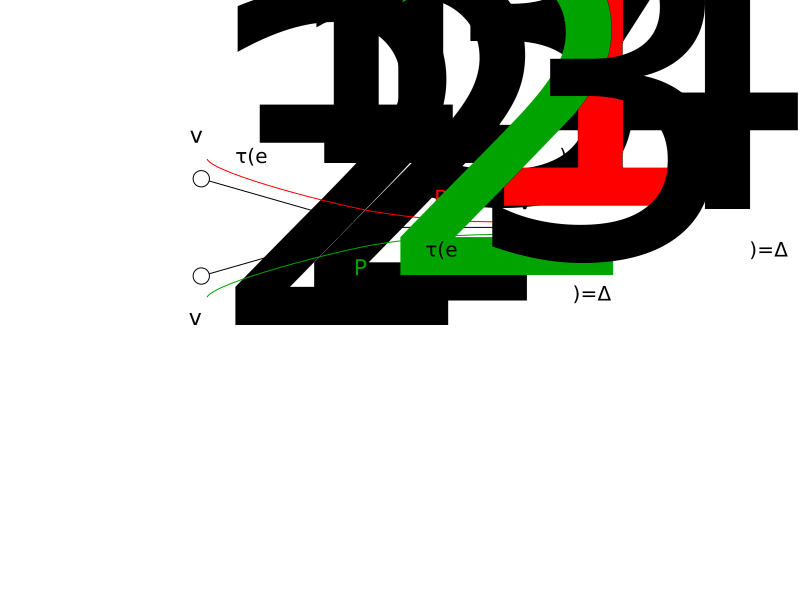
\includegraphics[width=0.5\textwidth]{ex_inc_time_1}}
    \subfloat{\usebox{\tempbox}}%
    \qquad
    \subfloat{\vbox to \ht\tempbox{%
      \vfil
        \begin{tabular}{ l| c c c c c }
          t (in $\Delta/2$) & 0 & 1 & 2 & 3 & 4 \\ \hline
          f($e_1$)          & \red{1} & 0 & 0 & 0 & 0 \\
          f($e_2$)          & \green{1} & 0 & 0 & 0 & 0 \\
          f($e_3$)          & 0 & \red{1} & \green{1} & 0 & 0 \\
          L($e_3$)          & 0 & 1 & 2 & 1 & 0
        \end{tabular}
      \vfil}}%
      \caption{Netzwerk, in dem ein maximaler Fluss sich beim Aufrunden staut;
        dazu ein Verlauf dieses maximalen Flusses}\label{fig:ex_inc_time_1}
    \end{figure}

    Die Tabelle in \figRef{ex_inc_time_1} gibt den Zeitverlauf eines maximalen Flusses
    $f$ an. $L$ ist dabei die Last auf einer Kante (der Fluss, der sich
    derzeit auf der Kante befindet).

    Wie man sieht, befinden sich zum Zeitpunkt $2$ zwei Flusseinheiten gleichzeitig
    auf $e_3$. Werden nun die Zeiten zu $\Delta$ aufgerundet, ergibt sich der
    Netzwerkausschnitt aus \figRef{ex_inc_time_2}.

    \begin{figure}[H]
    \centering
    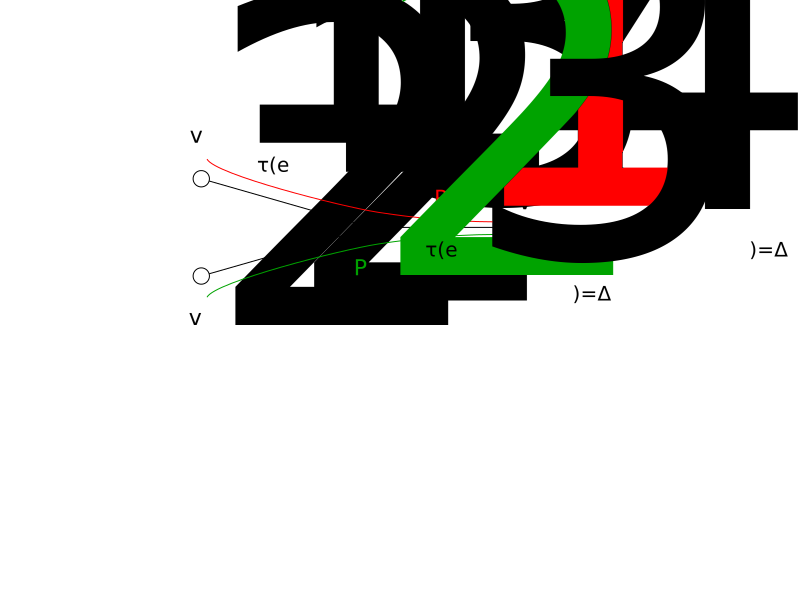
\includegraphics[width=0.5\textwidth]{ex_inc_time_2}
    \caption{Awesome Image}
    \label{fig:ex_inc_time_2}
    \end{figure}

     Überträgt man den Fluss $x$ nun
    in dieses Netzwerk, muss $x$ auf $e_1$ oder $e_2$ verzögert werden, da $P_1$
    und $P_2$ an dieser Stelle nicht gleichzeitig benutzt werden können.
    Auf $e_3$ „staut“ sich der Fluss.

    Insgesamt benötigt der Fluss dann $2\Delta$ statt lediglich $\frac{3}{2}\Delta$
    Zeiteinheiten.
\end{example}

Daraus ergibt sich die erste Bedingung, die an $(\graph, \tau)$ gestellt wird:
\begin{framed}
\begin{enumerate}[label={(A\arabic*)}]
    \item Die optimale Laufzeit in $(\graph, \widetilde{\tau})$ approximiert
        die optimale Laufzeit in $(\graph, \tau)$,
        d.h. $|\widetilde{T}^* - T^*| \leq \eps$,
        wenn $|\widetilde{\tau}(e) - \tau(e)| \leq \eps$. \label{a1}
        % BjH: Was bedeuten Stern und Tilde hier?
        % BjH: Hier ist mir noch nicht ganz klar. Entlang eines Pfades k\"onnten sich doch die Rundungen \"uber verschiedene Kanten aufsummieren.
\end{enumerate}
\end{framed}

\begin{example}

    Wir betrachten nun ein Netzwerk, in dem die Situation genau umgekehrt ist:
    im Netzwerk mit aufgerundeten Zeiten lässt sich ein viel besserer Fluss
    konstruieren, als im Originalnetzwerk. Wir betrachten dazu das Netzwerk
    in \figRef{ex_val_red_1}. Dort verlaufen alle Pfade $s-t$ über die
    Kante $e$. Wenn nun die Laufzeiten zu $\Delta$ aufgerundet werden,
    ergibt sich das Netzwerk in \figRef{ex_val_red_2}.

    \begin{figure}[H]
    \centering
    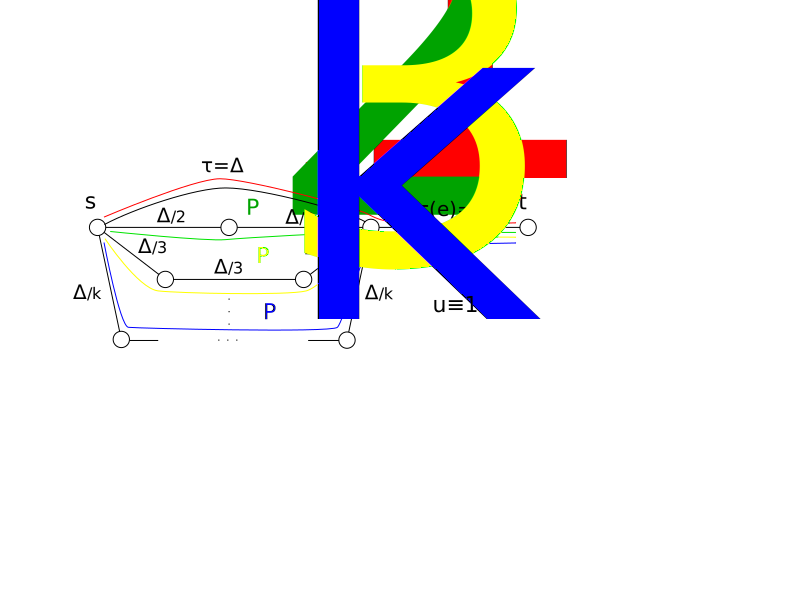
\includegraphics[width=0.6\textwidth]{ex_val_red_1}
    \caption{Awesome Image}
    \label{fig:ex_val_red_1}
    \end{figure}
    
    Man sieht, dass man einen Fluss $f$ auf allen Kanten gleichzeitig losschicken
    kann, dann kommt dieser versetzt am Knoten $v$ an. Siehe dazu auch
    $f(e)$ in der Tabelle. Soll dieser Fluss wieder im Originalnetzwerk
    interpretiert werden, muss fast der komplette Fluss verworfen werden, denn
    sonst wäre $f(e) = k > 1 = u(e)$, wenn $k > 1$.
    
    % \newsavebox{\tempbox}
    \begin{figure}[H]
    \sbox{\tempbox}{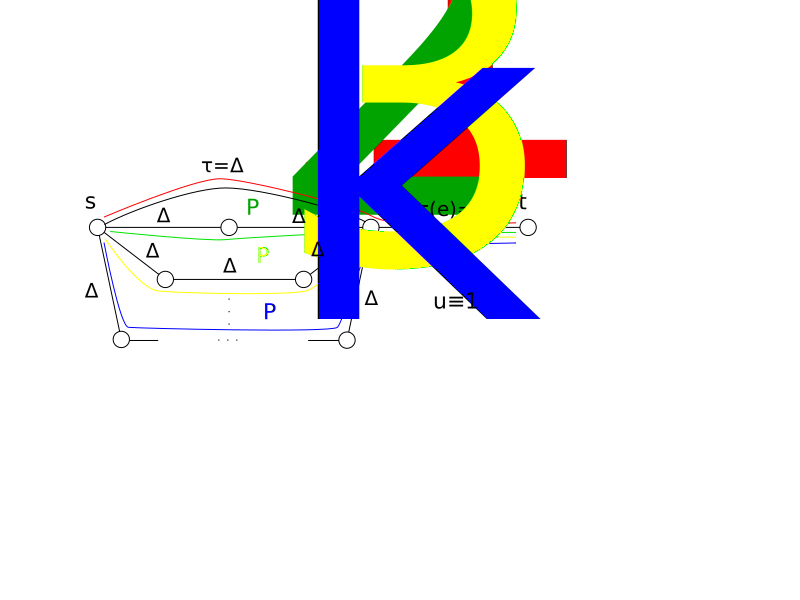
\includegraphics[width=0.5\textwidth]{ex_val_red_2}}
    \subfloat{\usebox{\tempbox}}%
    \qquad
    \subfloat{\vbox to \ht\tempbox{%
      \vfil
        \begin{tabular}{ l| c c c c c c c }
          t (in $\Delta/2$) & 0 & 1 & 2 & 3 & \ldots & k & \ldots \\ \hline
          f($P_1$)  & \red{1} & 0 & 0 & 0 & \ldots & \red{1} & \\
          f($P_2$)  & \green{1} & 0 & 0 & 0 & \ldots & \green{1} & \\
          f($P_3$)  & \yellow{1} & 0 & 0 & 0 & \ldots & \yellow{1} & \\
          \vdots    & \vdots & & & & & \vdots & \ldots \\
          f($P_k$)  & \blue{1} & 0 & 0 & 0 & \ldots & \blue{1} & \\
          f($e$)    & 0 & \red{1} & \green{1} & \yellow{1} & \ldots & \blue{1} &
        \end{tabular}
      \vfil}}%
      \caption{Netzwerk $(\graph, \tau')$, in dem nach Aufrunden ein viel größerer
        Fluss möglich ist}\label{fig:ex_val_red_2}
    \end{figure}    
\end{example}

Aus diesem Beispiel ergibt sich die zweite Bedingung:
\begin{framed}
\begin{enumerate}[start=2, label={(A\arabic*)}]
    \item Eine Lösung $\widetilde{f}$ in $(\graph, \widetilde{\tau})$ muss
        ohne großen Verlust in einen Fluss $f$ in $(\graph, \tau)$
        umgewandelt werden können: $||\widetilde{f}| - |f|| \leq \eps$.
        \label{a2}
\end{enumerate}
\end{framed}

Diese beiden Eigenschaften sind auch hinreichend für eine beliebig genaue
Approximation:
\begin{corollary}
    Sei $\graph$ ein Netzwerk mit zwei Laufzeiten $\tau_1$ und $\tau_2$, so dass
    \ref{a1} und \ref{a2} erfüllt sind.
    Dann kann ein optimaler Fluss $f_1^*$ in $(\graph, \tau_2)$ approximiert werden,
    wenn ein optimaler Fluss $f_2^*$ in $(\graph, \tau_2)$ approximiert werden kann.
    % BjH: Wo ist $\tau_1$ geblieben?

    \begin{proof}    
        Sei $\eps > 0$ und $\tau_2 - \tau_1 \leq \eps$ und seien
        $f_1^*$ und $f_2^*$ jeweils optimale Flüsse, die bei
        $T_1^*$ bzw. $T_2^*$ enden. Nach \ref{a1} ist $T_2^* - T_1^*\leq \eps$.

        Sei $f_2$ eine Approximation von $f_2^*$ in $(\graph, \tau_2)$ mit
        $||f_2| - |f_2^*|| \leq \eps$ und Ende $T_2 - T_2^* \leq \eps$.

        Dann kann $f_2$ als ein Fluss $f_1$ in $(\graph, \tau_1)$
        mit Ende $T_1$ interpretiert werden. Es gilt nach \ref{a2}:
        \begin{align*}
            ||f_1| - |f_1^*|| & \leq ||f_1| - |f_2^*| + \eps| \\
                            & \leq ||f_2| + \eps - |f_2^*| + \eps| \\
                            & \leq ||f_2| - |f_2^*|| + 2 \eps \\
                            & \leq 3 \eps
            % BjH: Sollte Epsilon hier nicht immer au\ss{}erhalb des Betrags stehen? Wenn die Differenz innerhalb des Betrags negativ ist, kann das Epsilon den Absolutwert verkleinern.
        \end{align*}
        und
        \begin{align*}
            T_1 - T_1^*  & \leq T_2 + \eps - T_2^* + \eps \\
                & \leq \eps + 2\eps \\
                & = 3 \eps
            % BjH: Hier und oben fehlen vermutlich die Betr\"age.
        \end{align*}
        
        Wähle als $\delta = \frac{\eps}{3}$. Dann kann $f_1^*$ in
        $(\graph, \tau_2)$ beliebig genau approximiert werden.
        % BjH: Was ist $\delta$?
    \end{proof}
\end{corollary}

%\begin{observation}
%    TODO: Beobachtung 5, zur Realisierung von \ref{a1} und \ref{a2} mit Speicher.
%\end{observation}


